\begin{figure}[t]
    \centering
    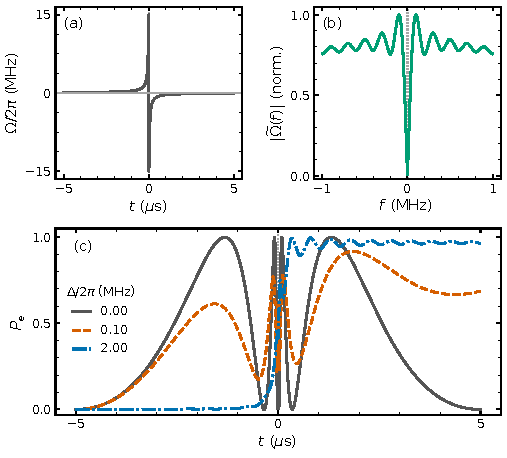
\includegraphics[width=0.88\columnwidth]{../figures/paper/01_pulse_mechanism.pdf}
    \caption{
    Pulse waveform and echo-cancellation mechanism.
    (a) Signed echo-root-Lorentzian drive envelope with peak amplitude $\Omega_0/(2\pi)=15~\mathrm{MHz}$ and a $\pi$ phase inversion at the pulse midpoint.
    (b) Normalized magnitude of the waveform Fourier spectrum, showing the spectral null at zero frequency produced by the phase inversion.
    (c) Unitary two-level excited-state population during the pulse at $\Delta/(2\pi)=0$, $0.10$, and $2.00~\mathrm{MHz}$, without relaxation or dephasing. At resonance, the evolution accumulated during the first half is exactly reversed during the second half, whereas finite detuning prevents complete cancellation.}
    \label{fig:fig1}
\end{figure}
